\clearpage
\appendix

\section{Notation}
\label{notation}
This section introduces the mathematical notations used throughout this document. It is taken from the book \citetitle{Goodfellow-et-al-2016} by \citeauthor{Goodfellow-et-al-2016} (\citeyear{Goodfellow-et-al-2016}).

\vspace{\notationgap}
% Need to use minipage to keep title of table on same page as table
\begin{minipage}{\textwidth}
	% This is a hack to put a little title over the table
	% We cannot use "\section*", etc., they appear in the table of contents.
	% tocdepth does not work on this chapter.
	\centerline{\bf Numbers and Arrays}
	\bgroup
	% The \arraystretch definition here increases the space between rows in the table,
	% so that \displaystyle math has more vertical space.
	\def\arraystretch{1.5}
	\begin{tabular}{cp{3.25in}}
		$\displaystyle a$ & A scalar (integer or real)\\
		$\displaystyle \va$ & A vector\\
		$\displaystyle \mA$ & A matrix\\
		$\displaystyle \tA$ & A tensor\\
		$\displaystyle \mI_n$ & Identity matrix with $n$ rows and $n$ columns\\
		$\displaystyle \mI$ & Identity matrix with dimensionality implied by context\\
		$\displaystyle \ve^{(i)}$ & Standard basis vector $[0,\dots,0,1,0,\dots,0]$ with a 1 at position $i$\\
		$\displaystyle \text{diag}(\va)$ & A square, diagonal matrix with diagonal entries given by $\va$\\
		$\displaystyle \ra$ & A scalar random variable\\
		$\displaystyle \rva$ & A vector-valued random variable\\
		$\displaystyle \rmA$ & A matrix-valued random variable\\
	\end{tabular}
	\egroup
	\index{Scalar}
	\index{Vector}
	\index{Matrix}
	\index{Tensor}
\end{minipage}

\vspace{\notationgap}
\begin{minipage}{\textwidth}
	\centerline{\bf Sets and Graphs}
	\bgroup
	\def\arraystretch{1.5}
	\begin{tabular}{cp{3.25in}}
		$\displaystyle \sA$ & A set\\
		$\displaystyle \R$ & The set of real numbers \\
		% NOTE: do not use \R^+, because it is ambiguous whether:
		% - It includes 0
		% - It includes only real numbers, or also infinity.
		% We usually do not include infinity, so we may explicitly write
		% [0, \infty) to include 0
		% (0, \infty) to not include 0
		$\displaystyle \{0, 1\}$ & The set containing 0 and 1 \\
		$\displaystyle \{0, 1, \dots, n \}$ & The set of all integers between $0$ and $n$\\
		$\displaystyle [a, b]$ & The real interval including $a$ and $b$\\
		$\displaystyle (a, b]$ & The real interval excluding $a$ but including $b$\\
		$\displaystyle \sA \backslash \sB$ & Set subtraction, i.e., the set containing the elements of $\sA$ that are not in $\sB$\\
		$\displaystyle \gG$ & A graph\\
		$\displaystyle \parents_\gG(\ervx_i)$ & The parents of $\ervx_i$ in $\gG$
	\end{tabular}
	\egroup
	\index{Scalar}
	\index{Vector}
	\index{Matrix}
	\index{Tensor}
	\index{Graph}
	\index{Set}
\end{minipage}

\vspace{\notationgap}
\begin{minipage}{\textwidth}
	\centerline{\bf Indexing}
	\bgroup
	\def\arraystretch{1.5}
	\begin{tabular}{cp{3.25in}}
		$\displaystyle \eva_i$ & Element $i$ of vector $\va$, with indexing starting at 1 \\
		$\displaystyle \eva_{-i}$ & All elements of vector $\va$ except for element $i$ \\
		$\displaystyle \emA_{i,j}$ & Element $i, j$ of matrix $\mA$ \\
		$\displaystyle \mA_{i, :}$ & Row $i$ of matrix $\mA$ \\
		$\displaystyle \mA_{:, i}$ & Column $i$ of matrix $\mA$ \\
		$\displaystyle \etA_{i, j, k}$ & Element $(i, j, k)$ of a 3-D tensor $\tA$\\
		$\displaystyle \tA_{:, :, i}$ & 2-D slice of a 3-D tensor\\
		$\displaystyle \erva_i$ & Element $i$ of the random vector $\rva$ \\
	\end{tabular}
	\egroup
\end{minipage}

\vspace{\notationgap}
\begin{minipage}{\textwidth}
	\centerline{\bf Linear Algebra Operations}
	\bgroup
	\def\arraystretch{1.5}
	\begin{tabular}{cp{3.25in}}
		$\displaystyle \mA^\top$ & Transpose of matrix $\mA$ \\
		$\displaystyle \mA^+$ & Moore-Penrose pseudoinverse of $\mA$\\
		$\displaystyle \mA \odot \mB $ & Element-wise (Hadamard) product of $\mA$ and $\mB$ \\
		% Wikipedia uses \circ for element-wise multiplication but this could be confused with function composition
		$\displaystyle \mathrm{det}(\mA)$ & Determinant of $\mA$ \\
	\end{tabular}
	\egroup
	\index{Transpose}
	\index{Element-wise product|see {Hadamard product}}
	\index{Hadamard product}
	\index{Determinant}
\end{minipage}

\vspace{\notationgap}
\begin{minipage}{\textwidth}
	\centerline{\bf Calculus}
	\bgroup
	\def\arraystretch{1.5}
	\begin{tabular}{cp{3.25in}}
		% NOTE: the [2ex] on the next line adds extra height to that row of the table.
		% Without that command, the fraction on the first line is too tall and collides
		% with the fraction on the second line.
		$\displaystyle\frac{d y} {d x}$ & Derivative of $y$ with respect to $x$\\ [2ex]
		$\displaystyle \frac{\partial y} {\partial x} $ & Partial derivative of $y$ with respect to $x$ \\
		$\displaystyle \nabla_\vx y $ & Gradient of $y$ with respect to $\vx$ \\
		$\displaystyle \nabla_\mX y $ & Matrix derivatives of $y$ with respect to $\mX$ \\
		$\displaystyle \nabla_\tX y $ & Tensor containing derivatives of $y$ with respect to $\tX$ \\
		$\displaystyle \frac{\partial f}{\partial \vx} $ & Jacobian matrix $\mJ \in \R^{m\times n}$ of $f: \R^n \rightarrow \R^m$\\
		$\displaystyle \nabla_\vx^2 f(\vx)\text{ or }\mH( f)(\vx)$ & The Hessian matrix of $f$ at input point $\vx$\\
		$\displaystyle \int f(\vx) d\vx $ & Definite integral over the entire domain of $\vx$ \\
		$\displaystyle \int_\sS f(\vx) d\vx$ & Definite integral with respect to $\vx$ over the set $\sS$ \\
	\end{tabular}
	\egroup
	\index{Derivative}
	\index{Integral}
	\index{Jacobian matrix}
	\index{Hessian matrix}
\end{minipage}

\vspace{\notationgap}
\begin{minipage}{\textwidth}
	\centerline{\bf Probability and Information Theory}
	\bgroup
	\def\arraystretch{1.5}
	\begin{tabular}{cp{3.25in}}
		$\displaystyle \ra \bot \rb$ & The random variables $\ra$ and $\rb$ are independent\\
		$\displaystyle \ra \bot \rb \mid \rc $ & They are conditionally independent given $\rc$\\
		$\displaystyle P(\ra)$ & A probability distribution over a discrete variable\\
		$\displaystyle p(\ra)$ & A probability distribution over a continuous variable, or over
		a variable whose type has not been specified\\
		$\displaystyle \ra \sim P$ & Random variable $\ra$ has distribution $P$\\% so thing on left of \sim should always be a random variable, with name beginning with \r
		$\displaystyle  \E_{\rx\sim P} [ f(x) ]\text{ or } \E f(x)$ & Expectation of $f(x)$ with respect to $P(\rx)$ \\
		$\displaystyle \Var(f(x)) $ &  Variance of $f(x)$ under $P(\rx)$ \\
		$\displaystyle \Cov(f(x),g(x)) $ & Covariance of $f(x)$ and $g(x)$ under $P(\rx)$\\
		$\displaystyle H(\rx) $ & Shannon entropy of the random variable $\rx$\\
		$\displaystyle \KL ( P \Vert Q ) $ & Kullback-Leibler divergence of P and Q \\
		$\displaystyle \mathcal{N} ( \vx ; \vmu , \mSigma)$ & Gaussian distribution %
		over $\vx$ with mean $\vmu$ and covariance $\mSigma$ \\
	\end{tabular}
	\egroup
	\index{Independence}
	\index{Conditional independence}
	\index{Variance}
	\index{Covariance}
	\index{Kullback-Leibler divergence}
	\index{Shannon entropy}
\end{minipage}

\vspace{\notationgap}
\begin{minipage}{\textwidth}
	\centerline{\bf Functions}
	\bgroup
	\def\arraystretch{1.5}
	\begin{tabular}{cp{3.25in}}
		$\displaystyle f: \sA \rightarrow \sB$ & The function $f$ with domain $\sA$ and range $\sB$\\
		$\displaystyle f \circ g $ & Composition of the functions $f$ and $g$ \\
		$\displaystyle f(\vx ; \vtheta) $ & A function of $\vx$ parametrized by $\vtheta$.
		(Sometimes we write $f(\vx)$ and omit the argument $\vtheta$ to lighten notation) \\
		$\displaystyle \log x$ & Natural logarithm of $x$ \\
		$\displaystyle \sigma(x)$ & Logistic sigmoid, $\displaystyle \frac{1} {1 + \exp(-x)}$ \\
		$\displaystyle \zeta(x)$ & Softplus, $\log(1 + \exp(x))$ \\
		$\displaystyle || \vx ||_p $ & $\normlp$ norm of $\vx$ \\
		$\displaystyle || \vx || $ & $\normltwo$ norm of $\vx$ \\
		$\displaystyle x^+$ & Positive part of $x$, i.e., $\max(0,x)$\\
		$\displaystyle \1_\mathrm{condition}$ & is 1 if the condition is true, 0 otherwise\\
	\end{tabular}
	\egroup
	\index{Sigmoid}
	\index{Softplus}
	\index{Norm}
\end{minipage}

Sometimes we use a function $f$ whose argument is a scalar but apply
it to a vector, matrix, or tensor: $f(\vx)$, $f(\mX)$, or $f(\tX)$.
This denotes the application of $f$ to the
array element-wise. For example, if $\tC = \sigma(\tX)$, then $\etC_{i,j,k} = \sigma(\etX_{i,j,k})$
for all valid values of $i$, $j$ and $k$.


\vspace{\notationgap}
\begin{minipage}{\textwidth}
	\centerline{\bf Datasets and Distributions}
	\bgroup
	\def\arraystretch{1.5}
	\begin{tabular}{cp{3.25in}}
		$\displaystyle \pdata$ & The data generating distribution\\
		$\displaystyle \ptrain$ & The empirical distribution defined by the training set\\
		$\displaystyle \sX$ & A set of training examples\\
		$\displaystyle \vx^{(i)}$ & The $i$-th example (input) from a dataset\\
		$\displaystyle y^{(i)}\text{ or }\vy^{(i)}$ & The target associated with $\vx^{(i)}$ for supervised learning\\
		$\displaystyle \mX$ & The $m \times n$ matrix with input example $\vx^{(i)}$ in row $\mX_{i,:}$\\
	\end{tabular}
	\egroup
\end{minipage}\clearpage

\section{Graph Networks}

\newlength{\threesubht}
\newsavebox{\threesubbox}
\begin{figure}[ht]
    \centering
    \sbox\threesubbox{
      \resizebox{\dimexpr.95\textwidth-1em}{!}{
        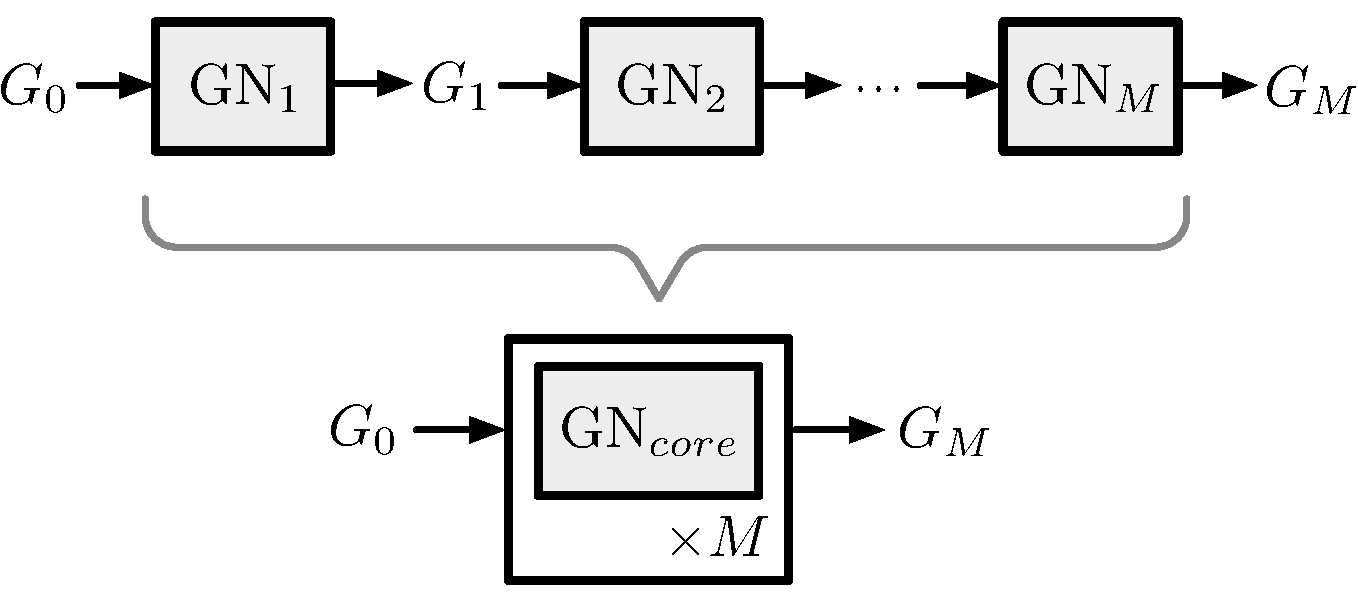
\includegraphics{resources/gn-stack-config}
        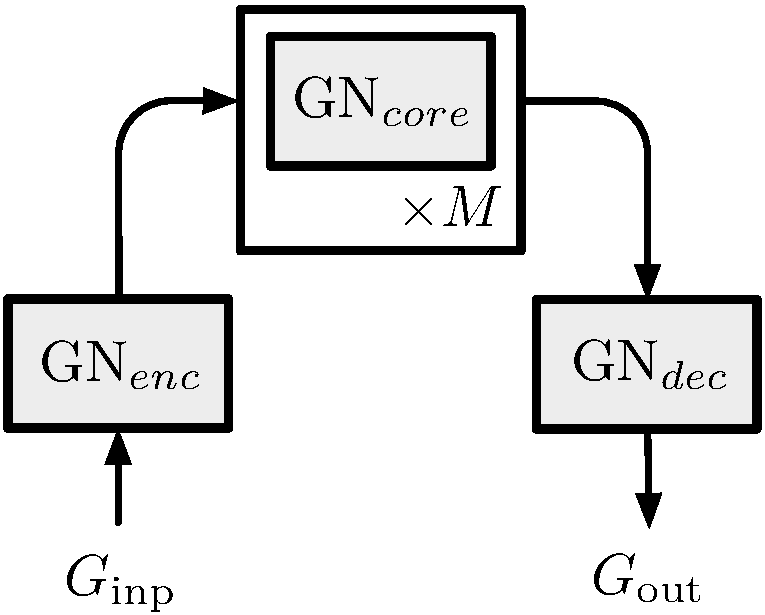
\includegraphics{resources/gn-epd-config}
        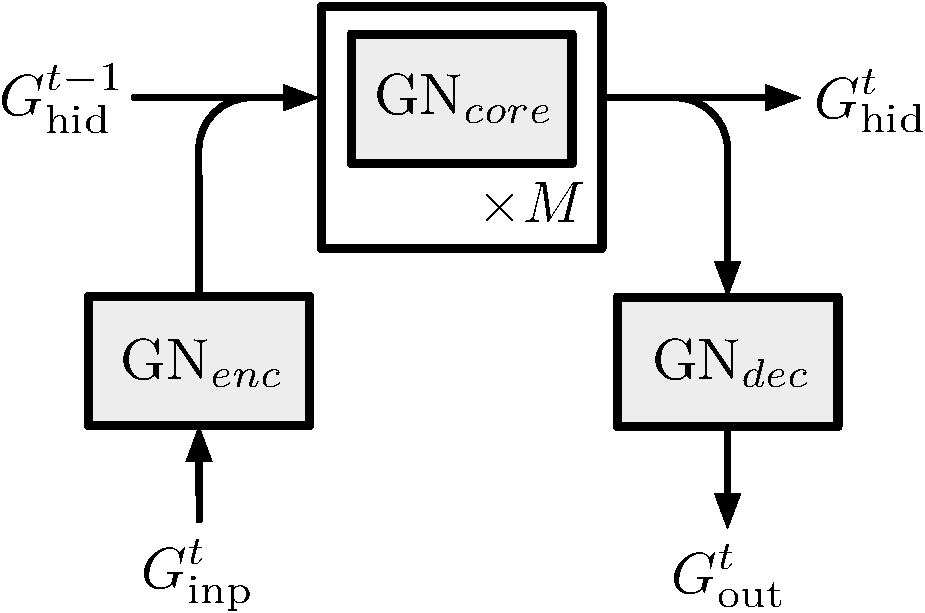
\includegraphics{resources/gn-rnn-config}
      }
    }
    \setlength{\threesubht}{\ht\threesubbox}
    \subcaptionbox{Composition of GN blocks\label{fig:gn-composition}}{%
      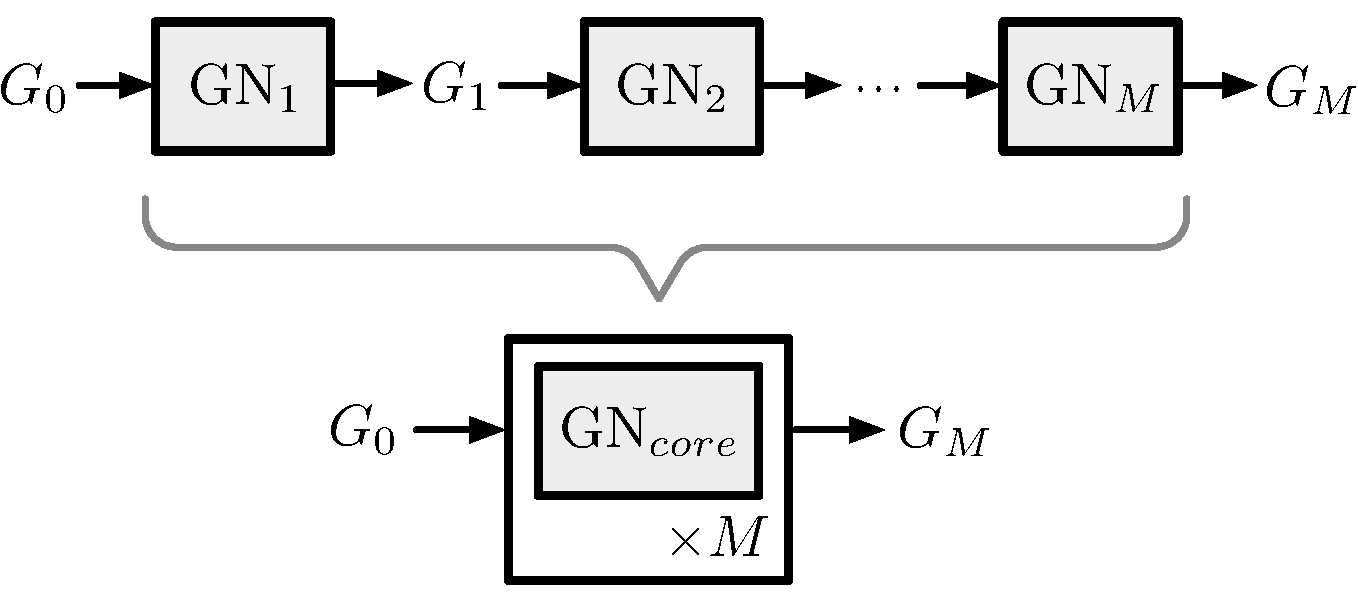
\includegraphics[height=1\threesubht]{resources/gn-stack-config}%
    }\quad
    \subcaptionbox{Encode-process-decode\label{fig:gn-epd-config}}{%
      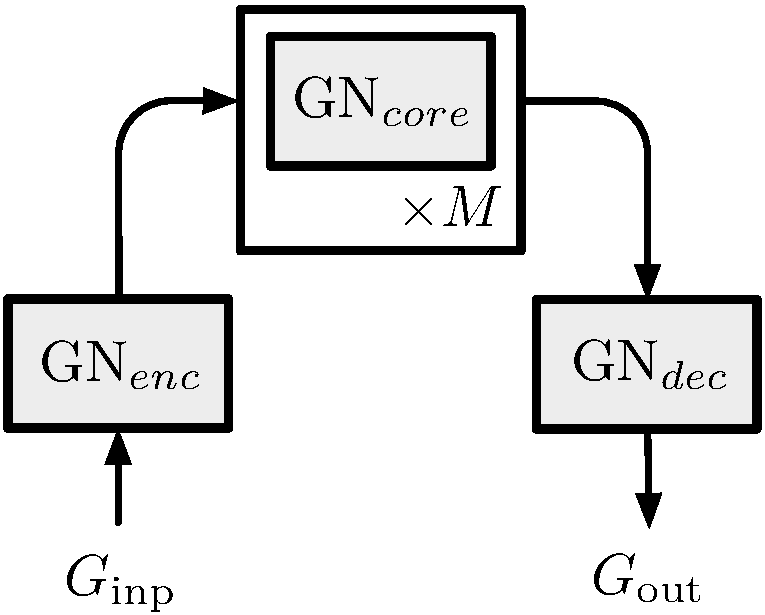
\includegraphics[height=1\threesubht]{resources/gn-epd-config}%
    }\quad
    \subcaptionbox{Recurrent GN architecture\label{fig:gn-rnn-config}}{%
      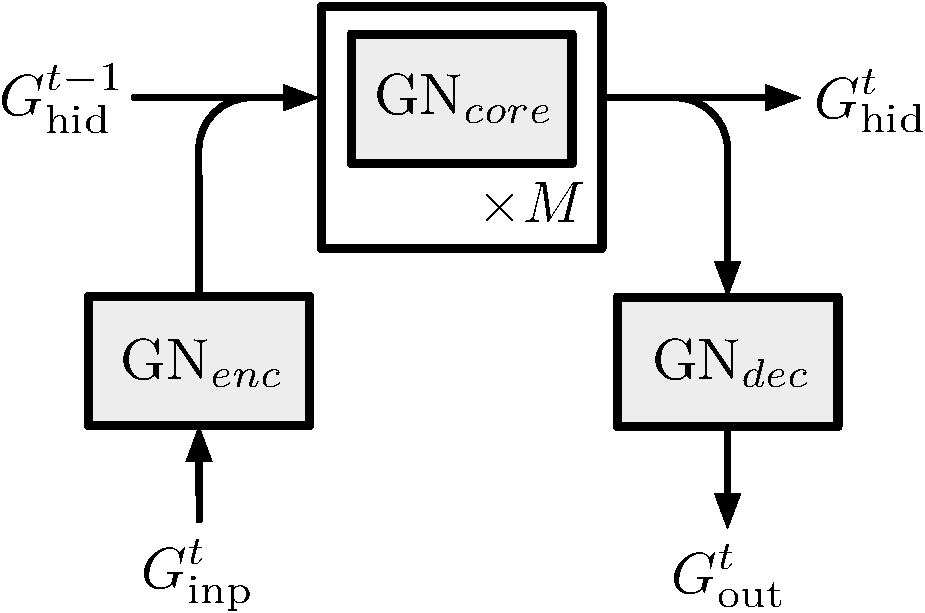
\includegraphics[height=1\threesubht]{resources/gn-rnn-config}%
    }
        \caption[GN block stacking methods: sequence, encode-process-decode, and recurrent encode-process-decode]{(a) An example composing multiple GN blocks in sequence to form a GN ``core''. Here, the GN blocks can use shared weights, or they could be independent. (b) The \emph{encode-process-decode} architecture, which is a common choice for composing GN blocks. Here, a GN encodes an input graph, which is then processed by a GN core. The output of the core is decoded by a third GN block into an output graph, whose nodes, edges, and/or global attributes would be used for task-specific purposes. (c) The encode-process-decode architecture applied in a sequential setting in which the core is also unrolled over time (potentially using a GRU or LSTM architecture), in addition to being repeated within each time step. Here, merged lines indicate concatenation, and split lines indicate copying. Source \cite{deepmind:graphnets}}
        \label{fig:gn-enc-proc-dec}
\end{figure}
\clearpage

\section{Dataset Samples}

\begin{figure}[h]
    \centering
    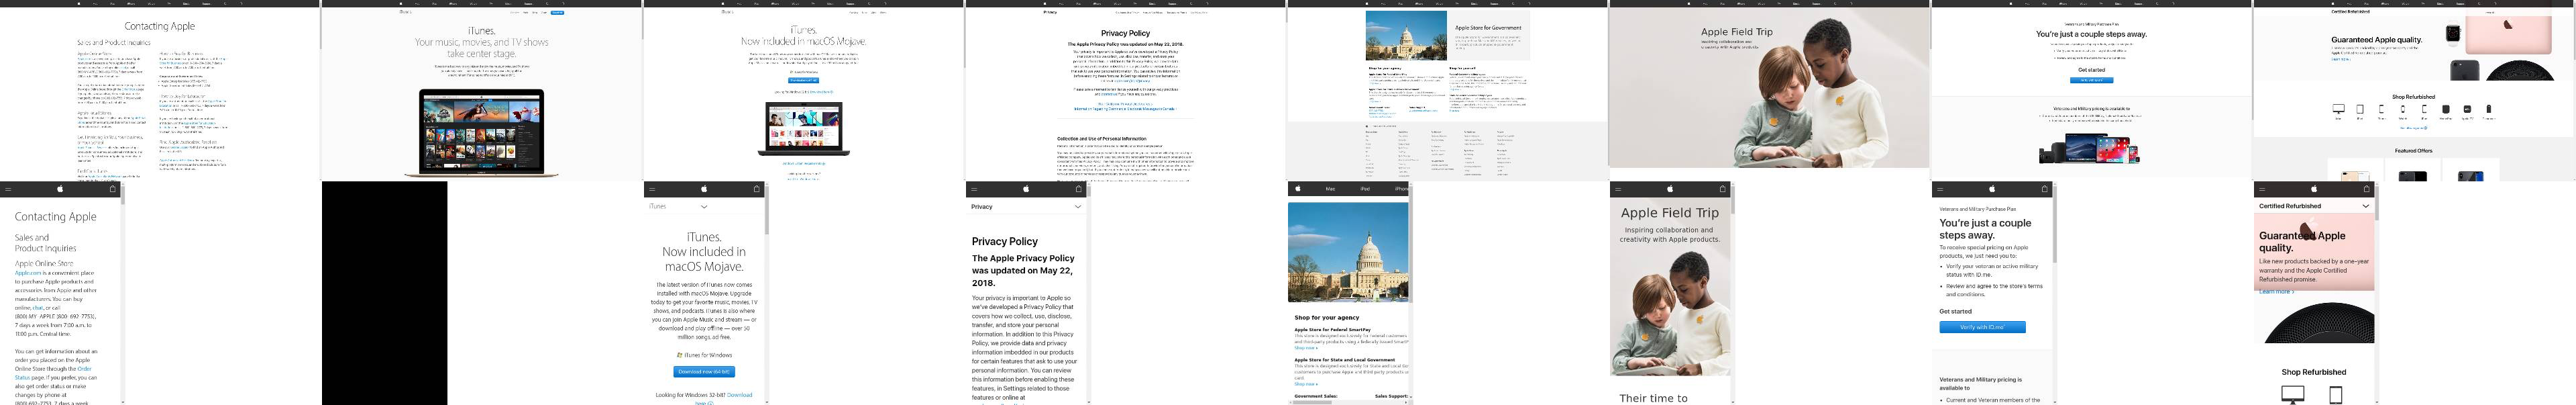
\includegraphics[clip,width=\columnwidth]{resources/dataset/v2-000011.png}\vspace{4mm}
    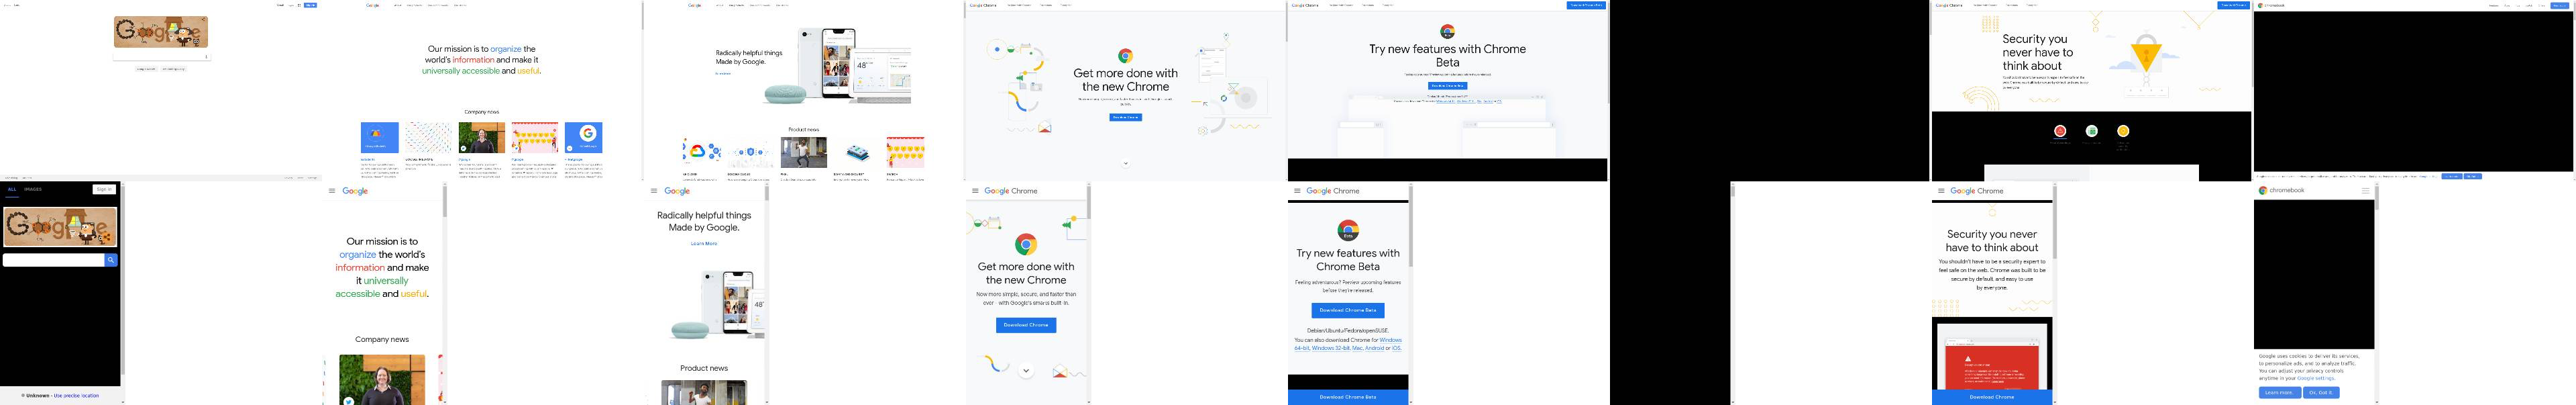
\includegraphics[clip,width=\columnwidth]{resources/dataset/v2-000100.png}\vspace{4mm}
    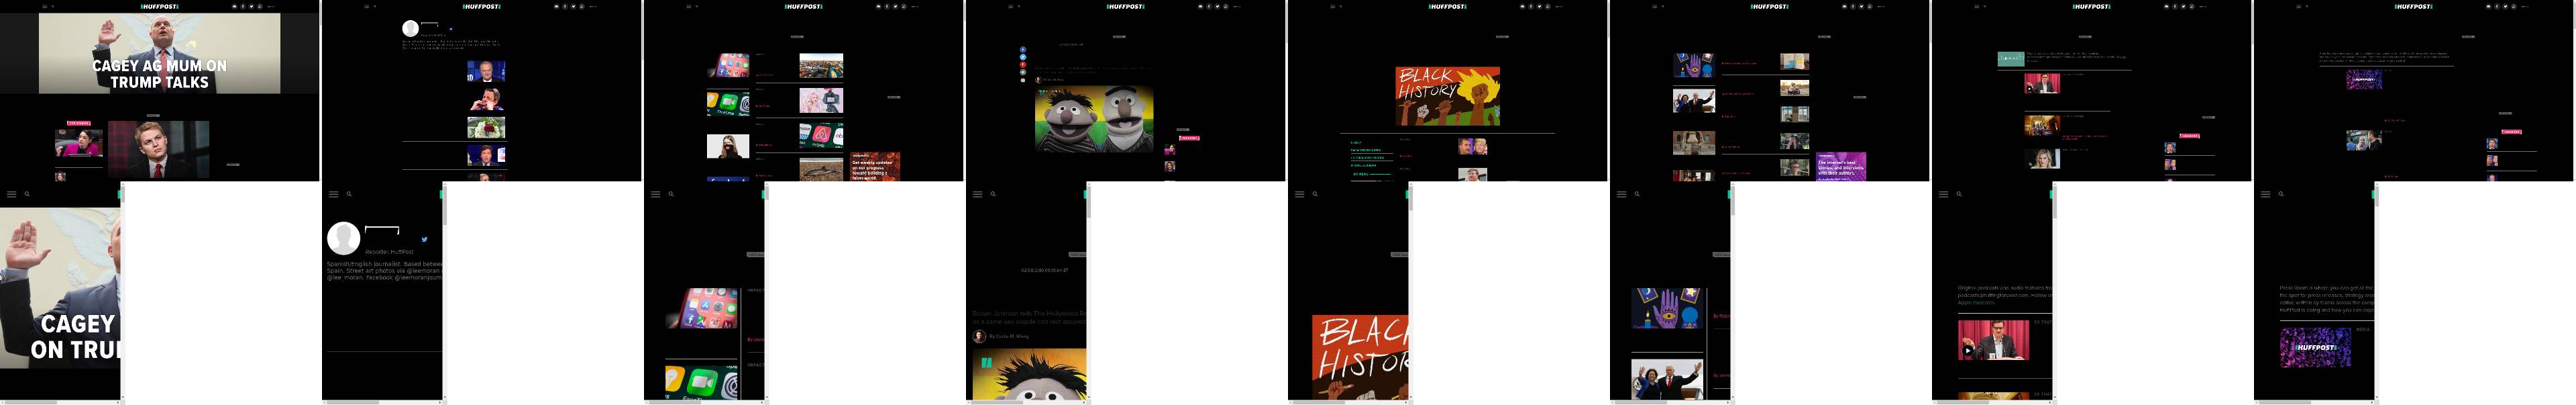
\includegraphics[clip,width=\columnwidth]{resources/dataset/v2-001000.png}\vspace{4mm}
    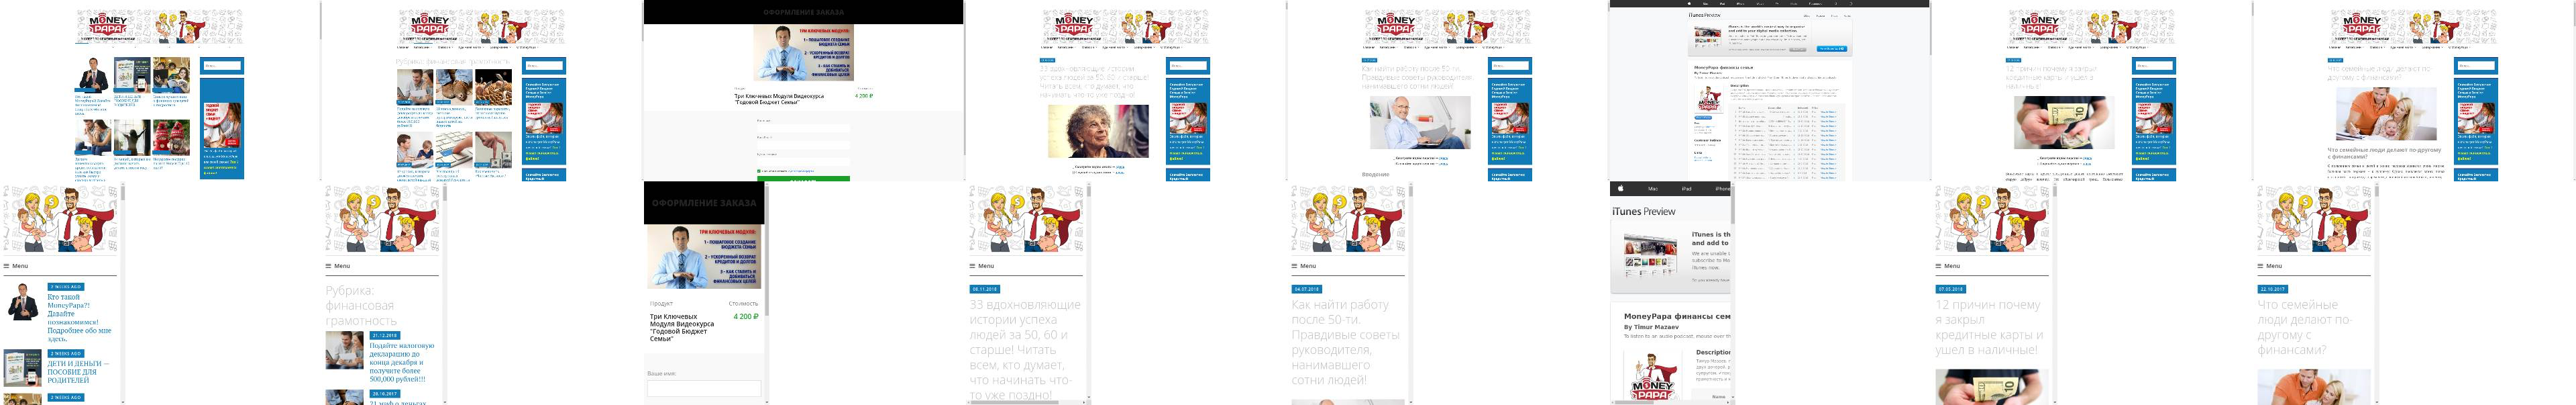
\includegraphics[clip,width=\columnwidth]{resources/dataset/v2-010000.png}\vspace{4mm}
    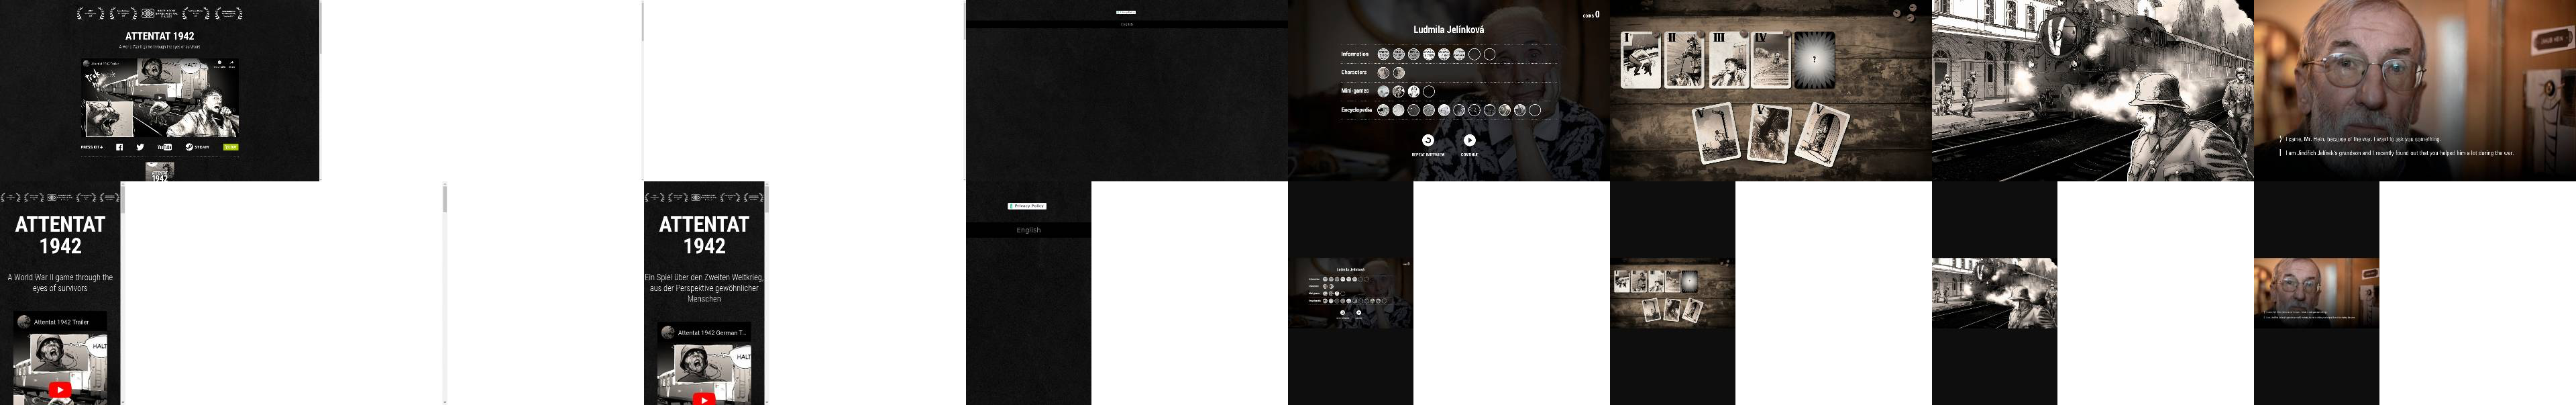
\includegraphics[clip,width=\columnwidth]{resources/dataset/v2-050000.png}\vspace{4mm}
    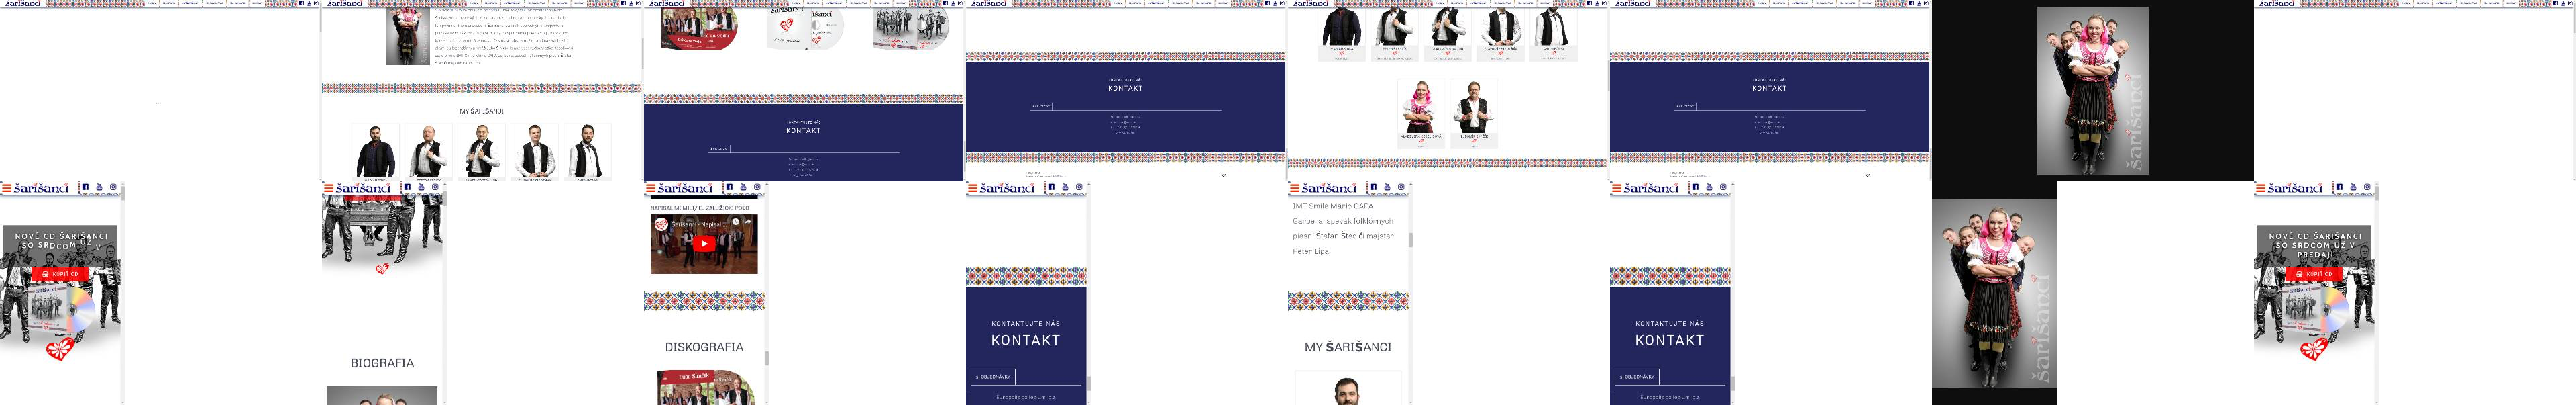
\includegraphics[clip,width=\columnwidth]{resources/dataset/v2-100000.png}
    \caption[Samples from dataset version 2]{Samples from dataset version 2 (desktop and mobile screenshots). Ranks, from top to bottom: \#11; \#100; \#1,000; \#10,000; \#50,000; \#100,000.}
    \label{fig:dataset samples}
\end{figure}\clearpage

\section{Source Code}

\begin{lstlisting}[
    label={lst:getthreefold},
    language=Python,
    caption={Dynamic and deterministic dataset splitting},
    captionpos=b
]
from collections import namedtuple
from typing import List, Type

Data = namedtuple('ThreefoldData', ['train', 'valid', 'test'])

def get_threefold(klass: Type, sample_paths: List[str], train_ratio: float, valid_ratio: float, logrank_b: float) -> Data:
    """
    :param klass: Dataset class, e.g. DatasetV2
    :param sample_paths: List of paths that point to the samples of the dataset
    :param train_ratio: Value in [0,1], ratio of training samples
    :param valid_ratio: Value in [0,1], ratio of validation samples
    :param logrank_b: Logrank base (makes the weighting steeper b --> 0, more linear b --> 10, or inverted b > 10)
    :return: Three datasets (train, validation, test)
    """

    assert train_ratio + valid_ratio <= 1., "Train and validation ratio must be less than or equal to 1."
    assert len(sample_paths) > 0, "No dataset samples found."

    sample_paths = sorted(sample_paths)

    train_paths, valid_paths, test_paths = [], [], []

    for path in sample_paths:
        n_train, n_valid, n_test = len(train_paths), len(valid_paths), len(test_paths)
        n_total = n_train + n_valid + n_test

        if n_total == 0 or n_train / n_total < train_ratio:
            train_paths.append(path)
        elif n_valid / n_total < valid_ratio:
            valid_paths.append(path)
        else:
            test_paths.append(path)

    return Data(
        train=klass(train_paths, logrank_b),
        valid=klass(valid_paths, logrank_b),
        test=klass(test_paths, logrank_b))
\end{lstlisting}
\clearpage

\section{Activation Maps}

\begin{figure}[ht]
    \centering
    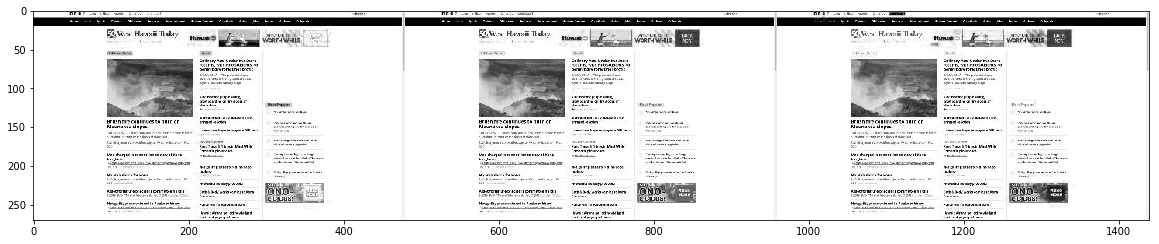
\includegraphics[clip,width=\columnwidth]{resources/analysis/feat-map-4058-0.png}\\
    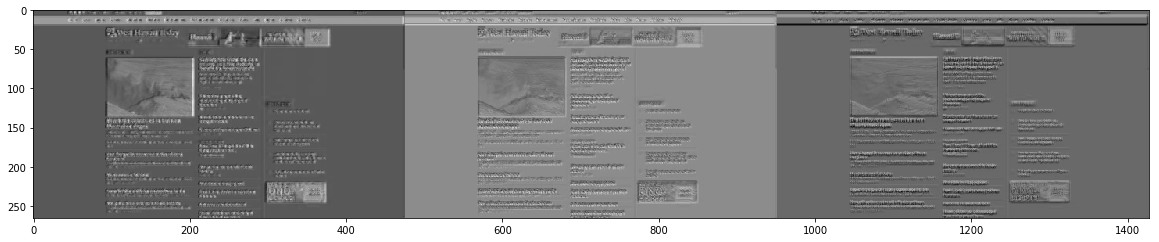
\includegraphics[clip,width=\columnwidth]{resources/analysis/feat-map-4058-1.png}\\
    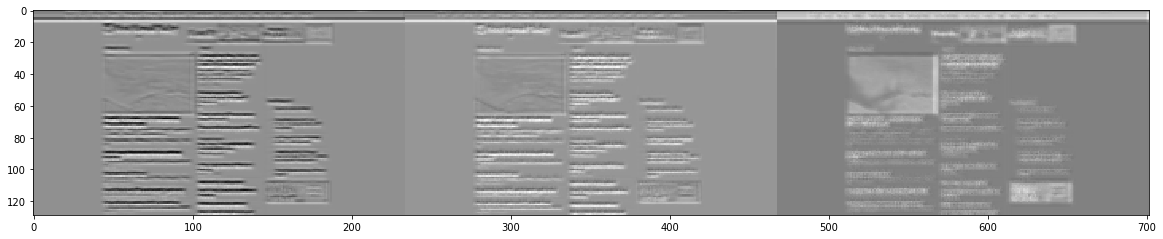
\includegraphics[clip,width=\columnwidth]{resources/analysis/feat-map-4058-2.png}\\
    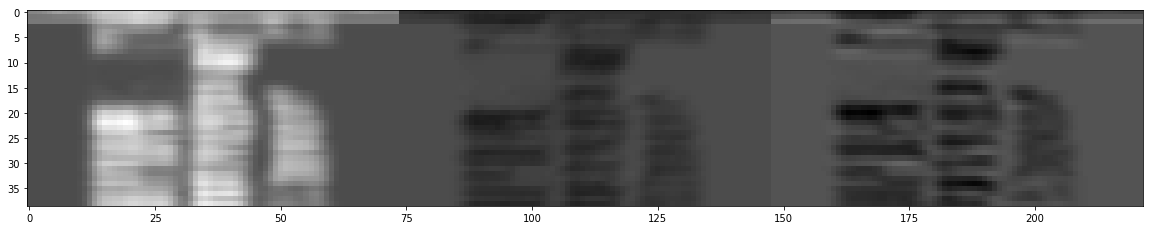
\includegraphics[clip,width=\columnwidth]{resources/analysis/feat-map-4058-3.png}\\
    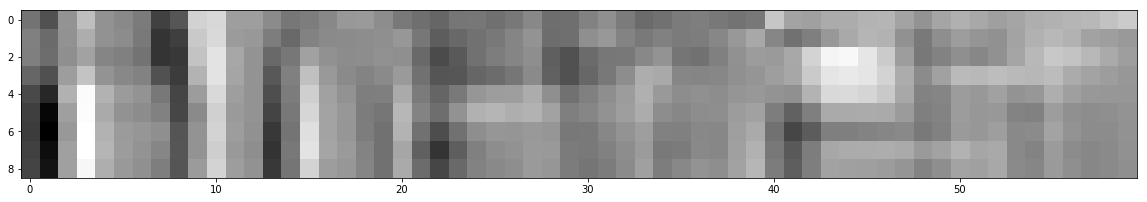
\includegraphics[clip,width=\columnwidth]{resources/analysis/feat-map-4058-4.png}\\
    \caption[Activation maps of the CNN for sample \#4058]{Cherry-picked activation maps of the CNN for sample \#4058. Top to bottom: Input, Block1, Block2, Block3, and Block4.}
    \label{fig:activationmaps2}
\end{figure}

\begin{figure}[ht]
    \centering
    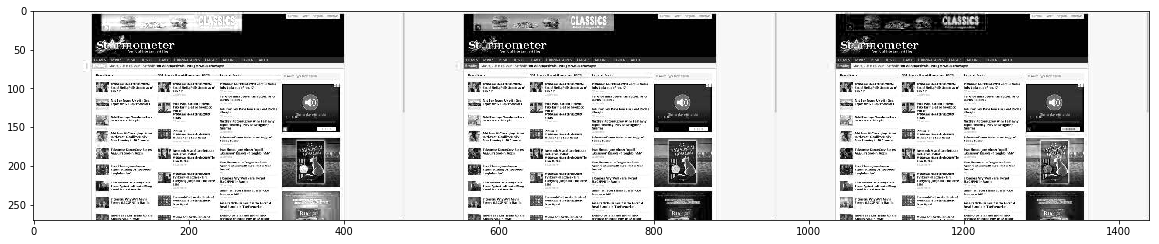
\includegraphics[clip,width=\columnwidth]{resources/analysis/feat-map-16364-0.png}\\
    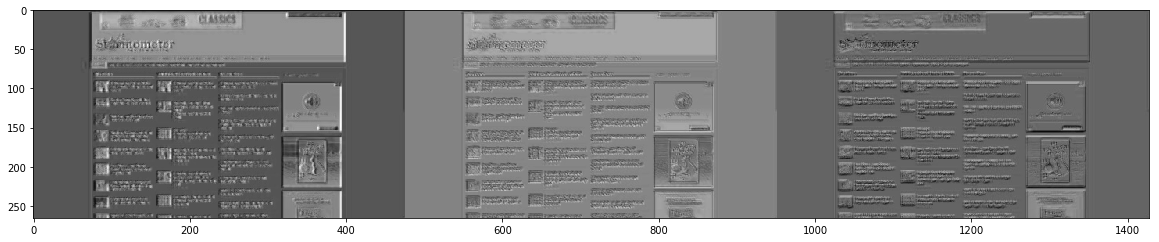
\includegraphics[clip,width=\columnwidth]{resources/analysis/feat-map-16364-1.png}\\
    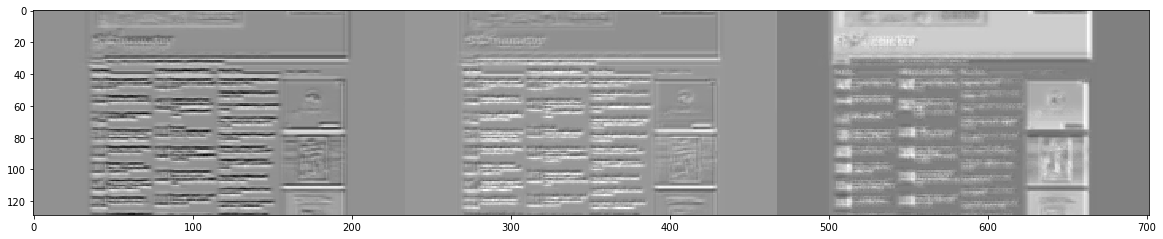
\includegraphics[clip,width=\columnwidth]{resources/analysis/feat-map-16364-2.png}\\
    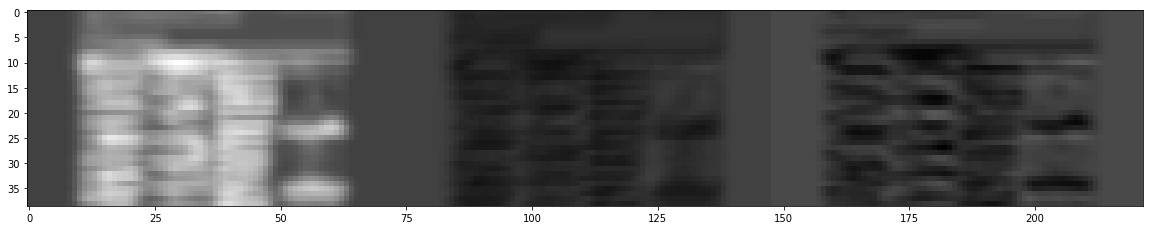
\includegraphics[clip,width=\columnwidth]{resources/analysis/feat-map-16364-3.png}\\
    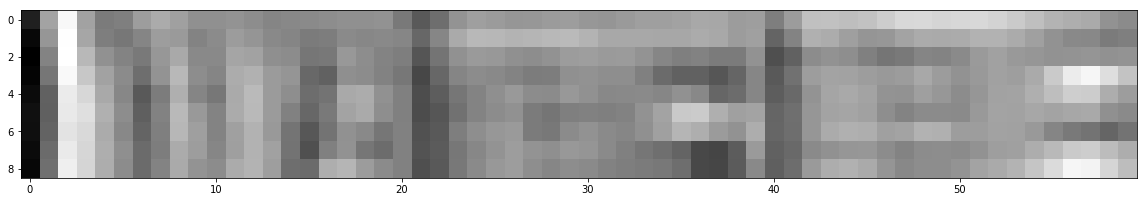
\includegraphics[clip,width=\columnwidth]{resources/analysis/feat-map-16364-4.png}\\
    \caption[Activation maps of the CNN for sample \#16364]{Cherry-picked activation maps of the CNN for sample \#16364. Top to bottom: Input, Block1, Block2, Block3, and Block4.}
    \label{fig:activationmaps3}
\end{figure}
\clearpage
